\chapter{Graphentheorie}
\label{chp:graphtheory}

Das Stromnetzwerk teilt sich aufgrund der starken Vernetzung die Eigenschaften mit Anwendungen von Graphvisualisierungen, wie zum Beispiel biologische Systeme, U-Bahn-Netzwerke und Dateisystemen. Aus diesem Grund werden die Grundlagen von Graphentheorie in diesem Kapitel erläutert.

\section{Grundlagen eines Graphen}

Graphen sind abstrakte mathematische Strukturen, die aus einer Menge von Knoten und den dazwischen verlaufenden Kanten bestehen. Jede Kante in einem Graphen repräsentiert eine Verbindung zwischen genau zwei Knoten. Die wissenschaftliche Disziplin, die sich mit der Untersuchung und Analyse solcher Graphen befasst, ist als Graphentheorie bekannt. In der Graphentheorie werden unterschiedliche Eigenschaften und Charakteristika von Graphen erforscht, wodurch sie als mächtiges Werkzeug in verschiedenen wissenschaftlichen, informatischen und ingenieurwissenschaftlichen Anwendungen dient. In diesem Kapitel werden verschiedene Eigenschaften von Graphen analysiert und mittels Abbildungen veranschaulicht. \cite{ohlbach2018graphen}
\section{Ausrichtung}

Die Besonderheit eines gerichteten Graphen ist die eindeutige Vorgabe der Kantenrichtung. Innerhalb dieses Graphen verbindet jede Kante präzise einen Anfangs- mit einem Endknoten und werden durch Pfeile repräsentiert, die eindeutig die Richtung der Beziehung zwischen diesen Knoten anzeigen. In der realen Welt könnten derartige gerichtete Verbindungen exemplarisch in einem sozialen Netzwerk und dessen \emph{Following}-System auftreten, da die Möglichkeit besteht, dass eine Person A einer Person B folgt, jedoch nicht zwangsläufig umgekehrt. \cite{ohlbach2018graphen}

\begin{figure}
    \centering
    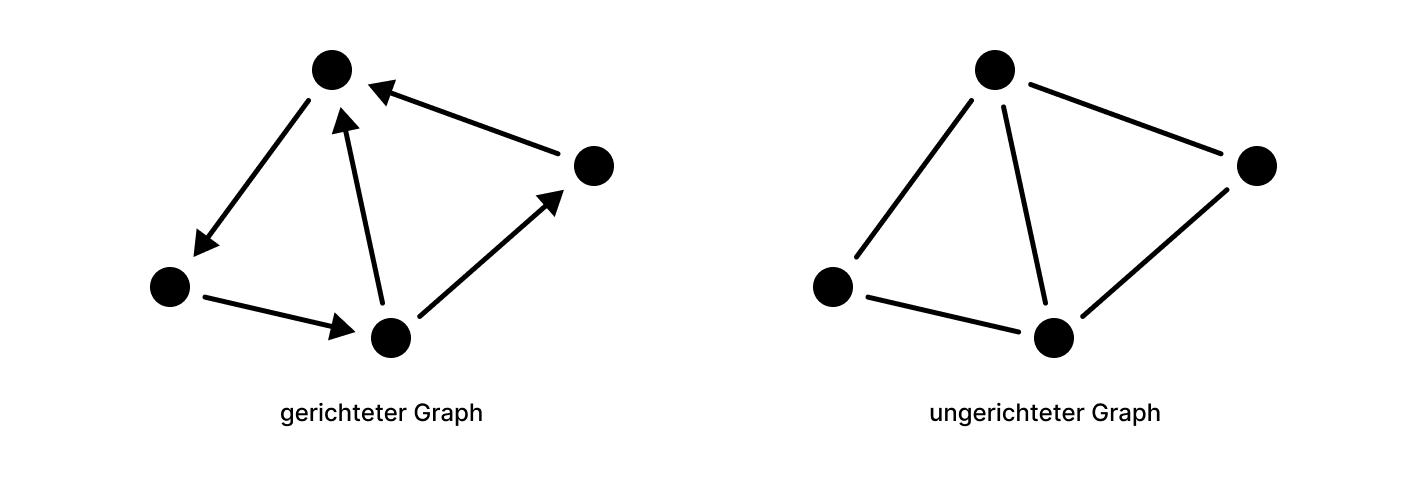
\includegraphics[width=1\textwidth]{content/img/Research/Graphen/Ausrichtung.png}
    \caption{Ein Graph mit gerichteten Kanten (links); ein Graph, dessen Kantenrichtung keine Bedeutung hat (rechts)}
    \label{fig:ausrichtung}
\end{figure}
\FloatBarrier
\section{Konnektivität}

Zusammenhängende Graphen haben die Eigenschaft keine Knoten aufzuweisen, welche vom Rest des Graphen isoliert sind. Diese Charakteristik impliziert das Fehlen isolierter Teilgraphen innerhalb des Gesamtgefüges. Die Gewährleistung der Zusammenhangseigenschaft bedeutet, dass sämtliche Knoten durch Pfade miteinander verbunden sind, wodurch der Graph als kohärente und nicht in isolierte Teile zerlegbare Einheit betrachtet wird. Nicht zusammenhängende Graphen können an ihren isolierten Knoten erkannt werden. \cite{kleinzusammenhang}

\begin{figure}
    \centering
    \includegraphics[width=1\textwidth]{content/img/Research/Graphen/Konnektivität.png}
    \caption{Ein Graph all dessen Knoten verbunden sind (links); ein Graph, welcher nicht verbundene Knoten enthält (rechts)}
    \label{fig:konnektivität}
\end{figure}
\FloatBarrier
\section{Zyklen}

Ein zyklischer Graph manifestiert sich durch die Existenz mindestens eines geschlossenen Pfades innerhalb seiner Struktur. Ein Pfad in diesem Sinne definiert sich als Abfolge von Kanten, dessen Anfangsknoten gleich dem Endknoten ist. Azyklisch wird ein Graph genannt, wenn seine Eigenschaften dem Gegenteil eines zyklischen Graphen entsprechen.

Die Ausführung von Algorithmen auf zyklischen Graphen erfordert besondere Achtsamkeit, da Zyklen potenziell zu komplexen, aufeinander abhängigen Situationen führen können. Das Ignorieren dieser Zyklen birgt das Risiko, dass solche Abhängigkeiten nicht aufgelöst werden. Daher ist eine präzise Analyse und Integration der zyklischen Strukturen in den algorithmischen Prozess unerlässlich, um die korrekte Verarbeitung von Daten und Abhängigkeiten zu gewährleisten. \cite{ohlbach2018graphen}

\begin{figure}
    \centering
    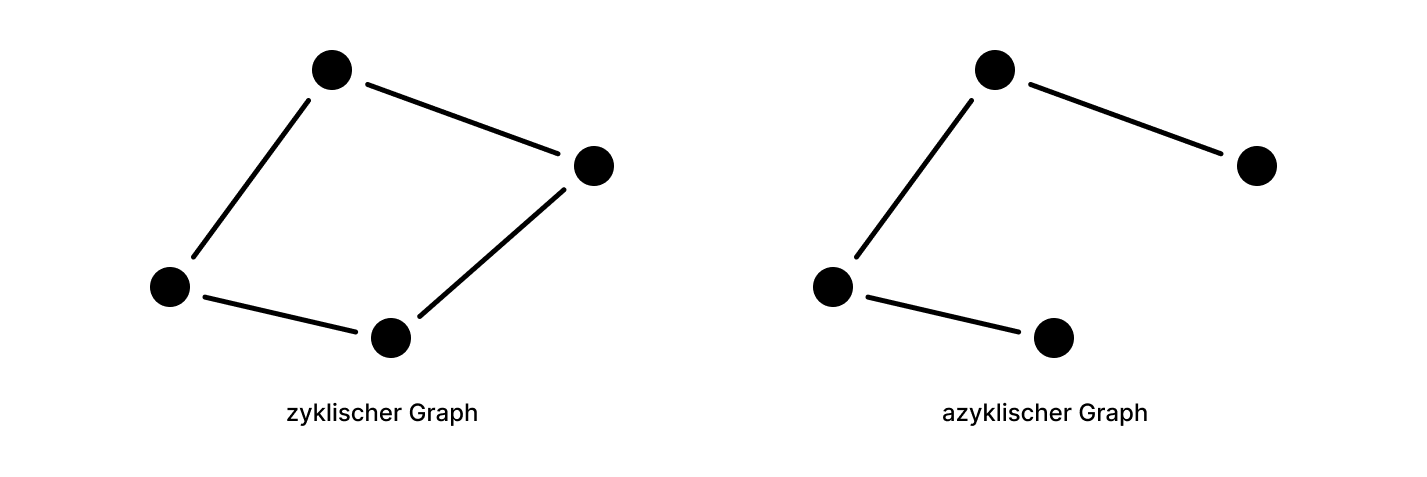
\includegraphics[width=1\textwidth]{content/img/Research/Graphen/Zyklen.png}
    \caption{Ein Graph, welcher einen geschlossenen Kreis (Zyklus) enthält (links); ein Graph ohne Zyklus (rechts)}
    \label{fig:zyklen}
\end{figure}
\FloatBarrier
\section{Gewicht der Kanten}

In einem gewichteten Graphen werden den Kanten zusätzliche numerische Werte zugeordnet, die als Gewichte bezeichnet werden. Diese Gewichte dienen dazu, verschiedene Arten von Beziehungen oder Kosten zwischen den Knoten zu repräsentieren. Die Gewichtung ermöglicht eine präzise Modellierung von unterschiedlichen Einflussstärken oder Ressourcenverbrauch entlang der graphentheoretischen Struktur, wie zum Beispiel Dauer und Länge einer Verbindungstrecke zweier Haltestellen bei einem öffentlichen Verkehrsnetzwerk. \cite{ohlbach2018graphen}

\begin{figure}
    \centering
    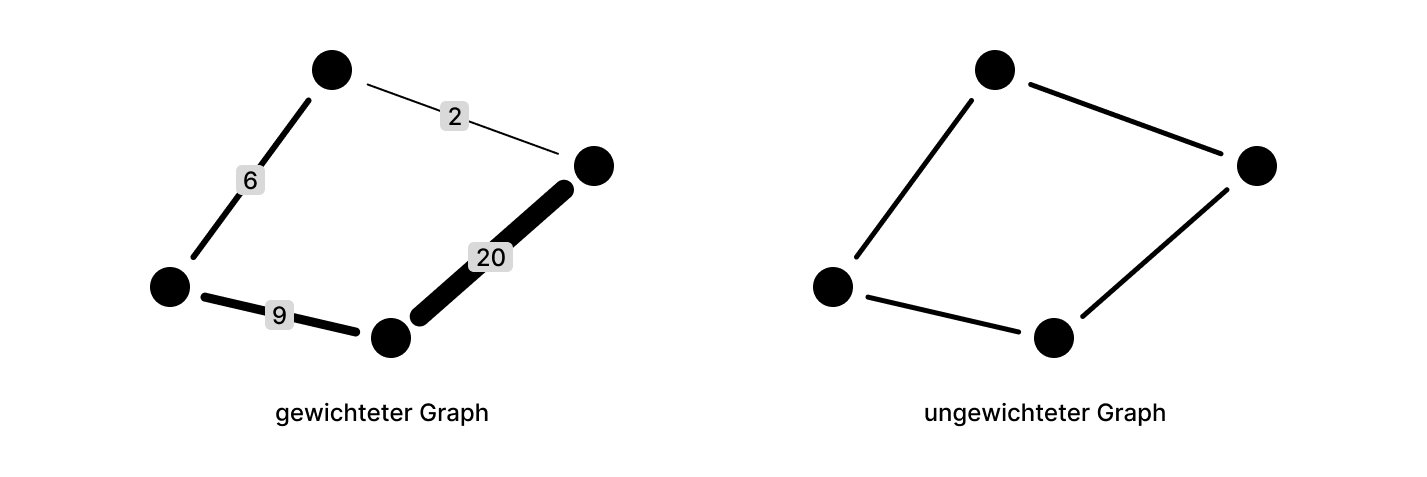
\includegraphics[width=1\textwidth]{content/img/Research/Graphen/Gewicht.png}
    \caption{Ein Graph, welcher gewichtete Kanten hat (links); ein Graph, dessen Kanten immer das gleiche Gewicht haben (rechts)}
    \label{fig:gewicht}
\end{figure}
\FloatBarrier
\section{Vollständigkeit}

Ein vollständiger Graph ist durch die Eigenschaft gekennzeichnet, dass jeder Knoten mit jedem anderen Knoten durch eine Kante verbunden ist. Diese charakteristische Vollständigkeit der Verbindungen impliziert eine maximale Interaktion zwischen den einzelnen Knoten des Graphen, wodurch sämtliche möglichen Kantenrelationen realisiert sind. Diese Einschränkung der Flexibilität von den Eigenschaften eines Graphen kommen aus diesem Grund seltener vor, weswegen die meisten Graphen unvollständig sind. \cite{ohlbach2018graphen}

\begin{figure}
    \centering
    \includegraphics[width=1\textwidth]{content/img/Research/Graphen/Vollständigkeit.png}
    \caption{Ein Graph, wo jeder Knoten mit allen anderen Knoten verbunden ist (links); nicht alle Knoten sind miteinander verbunden (rechts)}
    \label{fig:vollständigkeit}
\end{figure}
\FloatBarrier
\section{Bipartition}
\label{chp:bipartition}

Die Besonderheit eines bipartiten Graphen ist die Unterteilung aller Knoten in zwei disjunkte Mengen, wobei innerhalb beider Mengen keine Kanten existieren. Knoten dürfen dementsprechend nur miteinander verbunden sein, falls sich diese nicht in derselben Menge befinden. Allen nicht bipartiten Graphen fehlt es an solch einer Eigenschaft. \cite{ohlbach2018graphen}

\begin{figure}
    \centering
    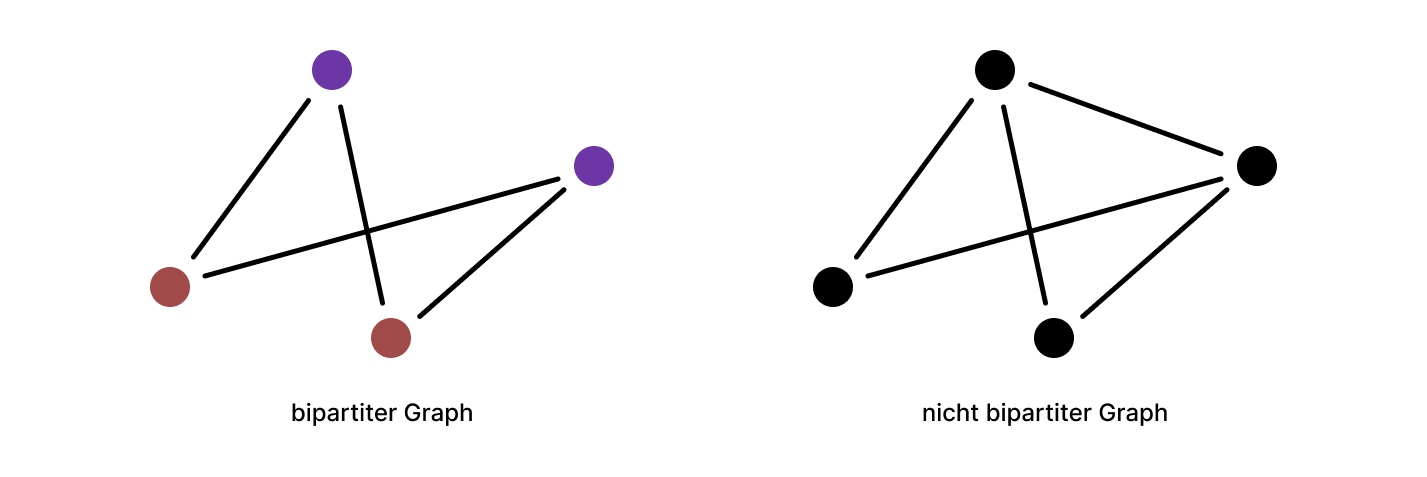
\includegraphics[width=1\textwidth]{content/img/Research/Graphen/Bipartition.png}
    \caption{Graph, welcher zwei Mengen ohne inhärente Verbindungen hat (links); keine Bipartition möglich beim rechten Graph}
    \label{fig:bipartition}
\end{figure}
\FloatBarrier
\section{Planarität}

Ein planarer Graph kann auf einer Ebene ohne Kantenkreuzungen dargestellt werden, was eine klare zweidimensionale Visualisierung ermöglicht. Im Gegensatz dazu erfordert ein nicht planarer Graph Kantenkreuzungen bei der Darstellung auf einer Ebene, was die visuelle Erfassung erschwert. Die Planarität beeinflusst somit nicht nur die Struktur, sondern auch die graphische Repräsentation und Analyse des Graphen \cite{lauchli1991planaritat,schmit2018kuratowski}. 

\begin{figure}
    \centering
    \includegraphics[width=1\textwidth]{content/img/Research/Graphen/Planarität.png}
    \caption{Ein Graph ohne Schnittpunkte der Kanten, wenn alle Knoten verbunden sind (links); nicht möglich ohne Schnittpunkte (rechts)}
    \label{fig:planarität}
\end{figure}
\FloatBarrier
\section{Eulerscher Graph}

Ein eulerscher Graph zeichnet sich durch die Existenz eines geschlossenen Pfades aus, der alle Kanten des Graphen genau einmal durchläuft. Diese charakteristische Eigenschaft ist als Eulerkreis bekannt und verleiht dem Graphen eine herausragende Struktur, da er eine systematische Durchquerung aller Verbindungen ermöglicht, ohne eine Kante zu wiederholen \cite{brandstadt1994eulerkreise,liebling1970euler}.

\begin{figure}
    \centering
    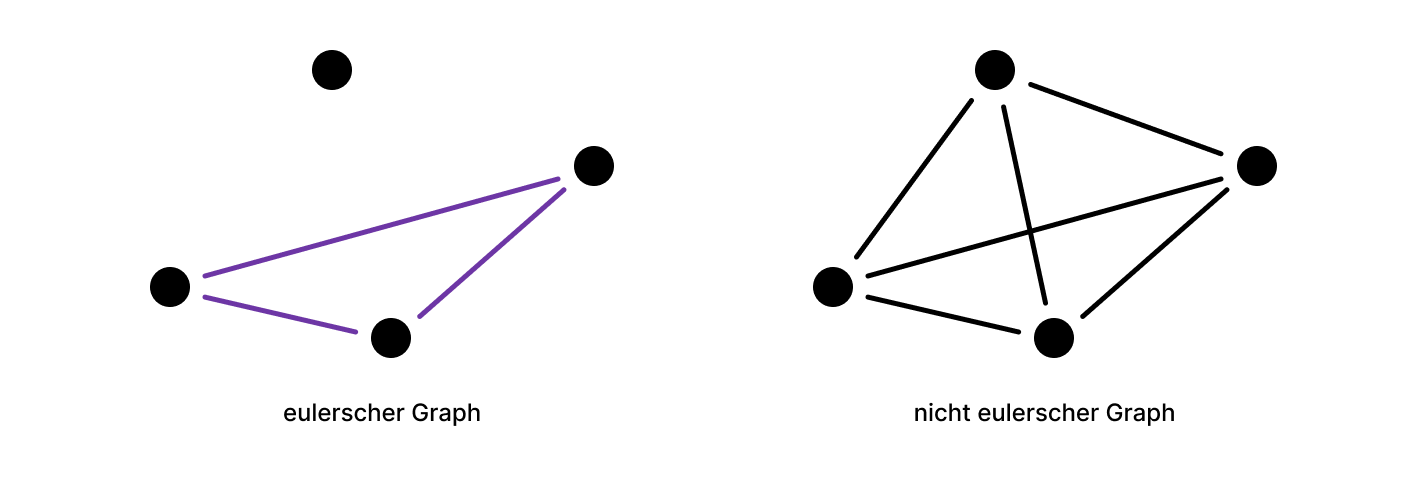
\includegraphics[width=1\textwidth]{content/img/Research/Graphen/EulerscherGraph.png}
    \caption{Graph mit einem Zyklus, welcher alle Kanten einmal enthält (links); Graph ohne diesen Eulerkreis (rechts)}
    \label{fig:eulersche}
\end{figure}
\FloatBarrier
\section{Hamiltonscher Graph}

Ein hamiltonscher Graph zeichnet sich durch die inhärente Eigenschaft aus, dass er die Existenz eines geschlossenen Pfades aufweist, welcher alle Knoten des Graphen exakt einmal durchläuft. Dieser geschlossene Pfad, bekannt als Hamiltonkreis, verankert die charakteristische Struktur des Graphen und ermöglicht eine vollständige, einmalige Durchquerung aller Knoten \cite{brandstadt1994eulerkreise, ohlbach2018graphen}.

Das Problem \emph{Hamilton} beschreibt das Finden eines solchen Pfades (auch Kreis). Dieses Problem hat die Eigenschaft keinen effizienten Algorithmus zu besitzen, jedoch kann eine potenzielle Lösung effizient auf ihre Richtigkeit überprüft werden. Aufgrund dieser Eigenschaft gehört Hamilton zur Klasse NP. Spezifischer ist Hamilton sogar ein \wordindoublequotes{NP-vollständiges Problem}, eine Klasse mit den schwierigsten Problemen der Mathematik.

\begin{quote}
    \say{Das Problem, einen Hamiltonschen Kreis in einem Graphen zu finden, bezeichnet man mit HAMILTON. Auch für dieses Problem ist kein effizienter Algorithmus bekannt.} - \textit{Steffen Reith}
    \cite{reith2001p}
\end{quote}

\begin{figure}
    \centering
    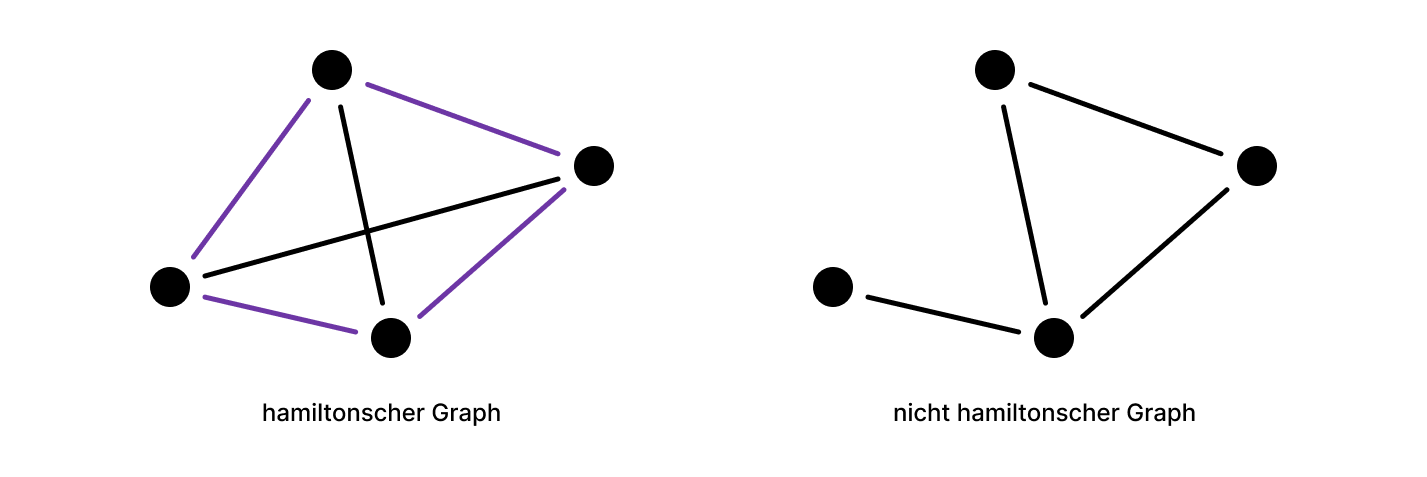
\includegraphics[width=1\textwidth]{content/img/Research/Graphen/HamiltonscherGraph.png}
    \caption{Graph mit Zyklus, welcher alle Knoten beinhaltet (links); kein Hamiltonscher Kreis möglich (rechts)}
    \label{fig:hamiltonsche}
\end{figure}
\FloatBarrier
Nachdem die Graphentheorie nun ausführlich erklärt wurde, widmen wir uns im nächsten Kapitel um die Visualisierung sowohl im Kontext der Benutzeroberfläche als auch im Kontext von stark vernetzten und komplexen Daten.